\documentclass[a4paper,14pt]{article}

\usepackage{comment} % Para comentar várias linhas ao mesmo tempo

%matemática
\usepackage{amsmath}
\usepackage{amssymb}

%diagramação
\usepackage{extsizes}
\everymath{\displaystyle}
\usepackage{geometry}
\usepackage{fancyhdr}
\usepackage{multicol}
\usepackage{graphicx}
\usepackage[brazil]{babel}
\usepackage[shortlabels]{enumitem}
\usepackage{cancel}
\usepackage{textcomp}
\usepackage{tcolorbox}

%tabelas
\usepackage{array} % Para melhor formatação de tabelas
\usepackage{longtable}
\usepackage{booktabs}  % Para linhas horizontais mais bonitas
\usepackage{float}   % Para usar o modificador [H]
\usepackage{caption} % Para usar legendas em tabelas
\usepackage{wrapfig} % Para usar tabelas e figuras flutuantes
\usepackage{xcolor} % Para cores do fundo de tabelas
\usepackage{colortbl} % Para cores do fundo de tabelas

%tikzpicture
\begin{comment}
	\usepackage{tikz}
	\usepackage{scalerel}
	\usepackage{pict2e}
	\usepackage{tkz-euclide}
	\usetikzlibrary{calc}
	\usetikzlibrary{patterns,arrows.meta}
	\usetikzlibrary{shadows}
	\usetikzlibrary{external}
\end{comment}


%pgfplots
\usepackage{pgfplots}
\pgfplotsset{compat=newest}
\usepgfplotslibrary{statistics}
\usepgfplotslibrary{fillbetween}

%colours
\usepackage{xcolor}



\columnsep=2cm
\hoffset=0cm
\textwidth=8cm
\setlength{\columnseprule}{.1pt}
\setlength{\columnsep}{2cm}
\renewcommand{\headrulewidth}{0pt}
\geometry{top=1in, bottom=1in, left=0.7in, right=0.5in}

\pagestyle{fancy}
\fancyhf{}
\fancyfoot[C]{\thepage}

\begin{document}
	
	\noindent\textbf{6FMA90 - Matemática} 
	
	\begin{center}Número de diagonais de um polígono convexo (Versão estudante)
	\end{center}
	
	\noindent\textbf{Nome:} \underline{\hspace{10cm}}
	\noindent\textbf{Data:} \underline{\hspace{4cm}}
	
	%\section*{Questões de Matemática}
	
	\begin{multicols}{2}
		\noindent O número de diagonais de um polígono convexo de $n$ lados é \\ $d = \frac{n(n - 3)}{2}$. \\
		\noindent\textsubscript{-----------------------------------------------------------------------}
		\begin{enumerate} 
			\item Usando uma régua, desenhe todas as diagonais do hexágono convexo. Quantas diagonais ele tem? \\\\\\\\\\
			\item Desenhe todas as diagonais do heptágono. Use a fórmula $d = \frac{n(n - 3)}{2}$ para verificar se você já desenhou todas. \\\\\\\\\\
			\item Calcule o número de diagonais de um: \\
			\begin{enumerate}[a)]
				\item hexágono \\\\\\\\\\
				\item triângulo \\\\\\\\\\
				\item quadrilátero \\\\\\\\\\
				\item eneágono \\\\\\\\\\
				\item dodecágono \\\\\\\\\\
				\item 100-ágono \newpage
			\end{enumerate}	
			\item Complete o quadro para os polígonos convexos. \\
			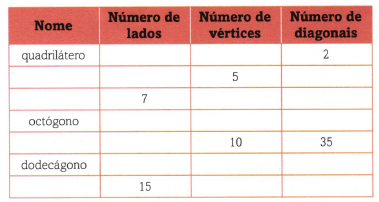
\includegraphics[width=1.1\linewidth]{6FMA90_imagens/imagem1}
			\textbf{Desafio olímpico} \\\\
			Se todos os quadradinhos são iguais, qual das figuras destacadas tem a menor área?
			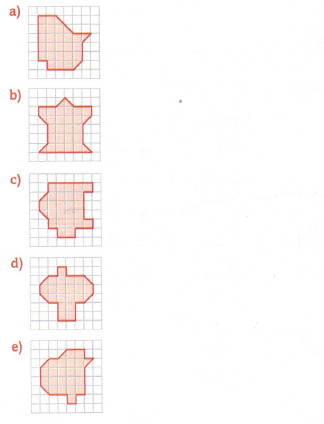
\includegraphics[width=1\linewidth]{6FMA90_imagens/imagem2}
			\item Quantas diagonais tem um:
			\begin{enumerate}[a)]
				\item heptágono? \\\\\\\\
				\item decágono? \\\\\\\\
				\item polígono de 13 lados? \\\\\\\\
				\item polígono de 16 lados? \\\\\\\\
				\item icoságono? \\\\\\\\
				\item polígono de 26 lados? \\\\\\\\
				\item pentadecágono? \\\\\\\\
				\item polígono de 31 lados? \\\\\\\\
			\end{enumerate}	
			\item Calcule o número de diagonais de um octógono. \\\\\\\\
			\item (FEI) O número de diagonais de um decágono convexo é:
			\begin{enumerate}[a)]
				\item 5
				\item 10
				\item 15
				\item 30
				\item 35
			\end{enumerate}	
		\end{enumerate}
		$~$ \\ $~$ \\ $~$ \\ $~$ \\ $~$ \\ $~$ \\ $~$ \\ $~$ \\ $~$ \\ $~$ \\ $~$ \\ $~$ \\ $~$ \\ $~$ \\ $~$ \\ $~$ \\ $~$ \\ $~$ \\ $~$ \\ $~$ \\ $~$ \\ $~$ \\ $~$ \\ $~$ \\ $~$ \\ $~$ \\ $~$ \\ $~$ \\ $~$ \\ $~$ \\ $~$ \\ $~$ \\ $~$ \\ $~$ \\ $~$ \\ $~$ \\ $~$ \\ $~$ \\ $~$ \\ $~$ \\ $~$ \\ $~$ \\ $~$ \\ $~$ \\ $~$ \\ $~$ \\ $~$ \\ $~$ \\ $~$ \\ $~$ \\ $~$ \\ $~$ \\ $~$ \\ $~$ \\ $~$ \\ $~$ \\ $~$ \\ $~$ \\ $~$ \\ $~$ \\ $~$ \\ $~$ \\ $~$ \\ $~$ \\ $~$ \\ $~$ \\ $~$ \\ $~$ \\ $~$ \\ $~$ \\ $~$ \\ $~$ \\ $~$ \\ $~$
	\end{multicols}
\end{document}